\documentclass[kulak]{kulakarticle} % options: kulak (default) or kul

\usepackage[dutch]{babel}
\usepackage{pdfpages}
\usepackage{graphicx}
\usepackage{mathtools}
\usepackage{nccmath}
\usepackage{cprotect}


\title{Smart Fire Extinguisher - Tussentijds Verslag}
\author{TEAM 6: Anna-Laura, Emile, Jérôme, Jesse}
\date{Academiejaar 2022 -- 2023}
\address{
	\textbf{Groep Wetenschap \& Technologie Kulak} \\
	Ingenieurswetenschappen \\
	P\&0 2}


\begin{document}

\maketitle



\section*{Inleiding}
                                          
Bij de brandbestrijding in grote warenhuizen worden momenteel \textbf{sprinklers} gebruikt. Deze zijn vastgemaakt aan het plafond van het gebouw en zijn aan de waterleiding aangesloten om bij brand water te doen neerdalen. Ze werken heel efficiënt, maar hebben wel enkele grote nadelen. De voornaamste zijn de kost van de aanleg en het onderhoud van alle leidingen die de sprinklers van water voorzien. Ook de verhoogde kans op waterschade bij het springen van een van de vele waterleidingen maakt sprinklers ietwat minder aantrekkelijk. Bovendien is het bestrijkingsgebied bij kleine branden niet proportioneel met de grootte van de brand waardoor er ook meer waterschade kan optreden dan nodig is. \\

Daarom zijn wij op zoek gegaan naar een efficiëntere manier om branden te blussen. Een \textbf{Smart Fire Extinguisher}, die zelf de branden kan detecteren, lokaliseren en gericht kan blussen. Zo zou 1 apparaat (met dus maar 1 aansluiting op de waterleiding of een eigen waterreservoir) een groot oppervlakte brandveilig kunnen maken. Dit zou het veel goedkoper maken voor de eigenaar die geen eindeloos lange waterleidingen moet aanleggen en onderhouden. De totale kost voor grote warenhuizen zou dus veel lager liggen en de kans op waterschade bij het springen van waterleidingen is veel kleiner.



\section{Ontwerp}
\subsection{Klantenvereisten}

De klant verwacht een apparaat dat zelfstandig branden kan detecteren en deze kan blussen. Hiervoor moet het de exacte locatie van de brand kunnen vaststellen en de arm in de juiste richting richten. Het apparaat moet water vanuit een jerrycan in de richting van de brand spuiten en zelf stoppen wanneer de brand geblust is. 

Alles moet automatisch werken, maar er moet ook een manuele override zijn waarbij het apparaat volledig manueel kan worden bestuurd en worden uitgeschakeld. Al dit moet gebeuren in communicatie met een PC. 



\subsection{Ontwerpspecificaties}
\begin{itemize}
	\item Branden detecteren en blussen in een rechthoek van 7m x 6m op 3m afstand 
	\item Maximale uitwijking horizontaal: 90°  
	\item Maximale uitwijking verticaal: 90°
	\item Hoeveelheid water per blussing: (wordt nog bekend gemaakt, foutenmarge nog inrekenen) 
	\item Hoeveelheid beschikbaar water: 10L 
	\item Elektronica afgeschermd van water 
	\item Massa robot: max. 20 kg
	\item Besturing via laptop
	\item Automatische werking
\end{itemize}

\subsection{Ontwerp}
We opteren voor een \textbf{stationair brandblusplatform} dat gebruik maakt van een draaiend platform en een arm om het water in de juiste richting en onder de juiste hoek weg te spuiten. Water uit een waterreservoir zal dan met behulp van een pomp op de gewenste plaats terecht komen. De plaats zal zijn vastgesteld door een camera. Deze detecteert de brand en aan de hand van de beelden zal er berekend worden waar en hoe ver de brand zich bevindt ten opzichte van het brandblusplatform. Daarna zullen nog een hoop berekeningen de hoek van de arm bepalen. \\

Voor de \textbf{detectie} van de brand maken we gebruik van een webcam (USB Webcam 1080P), in Python wordt een programma geschreven op een laptop die aan branddetectie en -lokalisatie doet. De camera is vastgemaakt op het roterend platform. \\

Het \textbf{richten} van het draaiend platform en de arm gebeurt met behulp van twee motoren (Micro Metal Gear Motor 100:1 HP), deze zullen dankzij een motor driver met de gewenste snelheid en in de juiste richting draaien. Volgens de berekeningen gedaan door een laptop en webcam zullen de armen juist gepositioneerd worden. De motoren worden bestuurd door een microcontroller (Arduino nano 33 iot). \\

Wanneer de arm correct gericht is, is de laatste stap het \textbf{blussen} van de brand. Hiervoor zal de pomp (Membraanpomp 12V 4.8 bar) water uit het waterreservoir (jerrycan 10L) door een slang (met diameter 10mm) pompen, om zo weggespoten te worden richting het doelwit. De benodigde afstand halen om het volledige bestrijkingsgebied te kunnen bestrijken is mogelijk door het aanpassen van het mondstuk.\\
%moet er in nog meer detail beschreven worden welke materialen we gebruiken en voor wat??

\begin{figure} [!h]
	\centering
	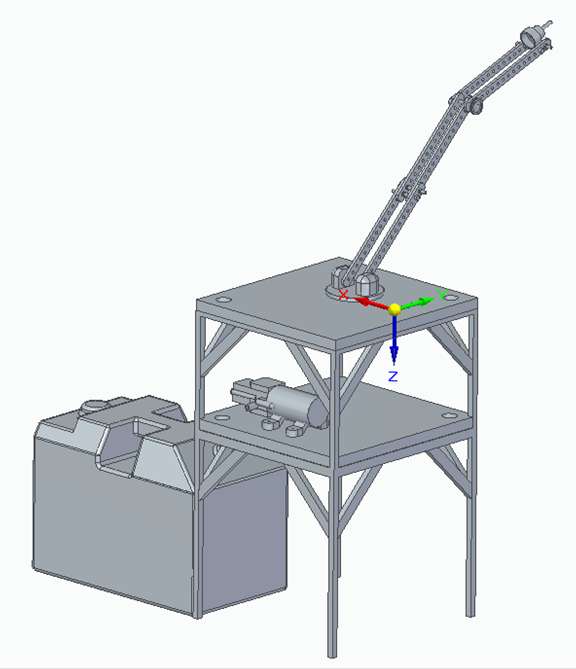
\includegraphics[width = .6 \textwidth]{Solid Edge Assembly foto}
	\caption{Ontwerp in Solid Edge}
	\label{ontwerp}
\end{figure}



\section{Berekeningen en code}
\subsection{Hoek van de waterstraal}
\subsubsection{Berekening}
De afstand zoals te zien in afbeelding \ref{schematische voorstelling} tussen het brandblusapparaat en de cilinder is \(x\) waarbij \(x\) maximaal gelijk kan zijn aan \(10,45 m\).
\begin{equation}
	x^2 = 3^2 + 10^2
	\Rightarrow x \approx 10,45 
\end{equation}
Om deze afstand te halen berekenen we de hoek waaronder het water moet worden weggespoten. De hoogte van het platform is hier \(h_1\) en de hoogte van de arm is \(h_2 = lsin(\theta)\) met \(l\) de lengte van de arm. \(y\) is de hoogte van de cilinder die moet worden opgevuld. Dan krijgen we:
\begin{equation}
	\begin{cases}
		x  = cos(\theta) v t \\
		y = h_1 + h_2 + sin(\theta) v t + \frac{-1}{2} g t^2
	\end{cases}
\end{equation}
Bij het gebruik van de brandblusser zullen we met behulp van de camera \(x\) al kennen, dankzij de waterflowsensor zullen we \(v\) ook accuraat kennen, \(h_1\) staat vast en \(h_2\) hangt af van de hoek \(\theta\). Uit de twee vergelijkingen kunnen we \(\theta\) en \(t\) halen en zal het doelwit gevuld geraken.

\subsubsection{Code}
De functie \verb*|hoekV(waterDebiet,afstandBeker)| (zie figuur \ref{flowchart_water}) berekent de hoek \(\theta\)  die nodig is tussen het platform en de arm. Deze functie heeft daarvoor het waterdebiet, in \(l/min\), nodig en de verticale afstand, in \(m\), tot het doelwit. Het waterdebiet wordt meegegeven door de waterflowsensor en de afstand door de webcam. Er worden ook niet-variabele parameters gebruikt die op voorhand zijn vastgelegd, zoals de straal van het spuitgat, de hoogte van het platform, de lengte van de arm, de hoogte van het doelwit en de afstand tussen het beginpunt van de arm en de camera. 

In deze functie wordt dan de snelheid van het water berekend en dat wordt in een stelsel gebruikt met twee vergelijkingen. Dit stelsel wordt, met gebruik van de scipy-package, opgelost naar de hoek \(\theta\) en de tijd \(t\).
\begin{equation}
	\begin{cases}
		afstandBeker  = cos(\theta )*lengteArm - afstandCamera + cos(\theta )*snelheid*t \\ 
		hoogteBeker  =  hoogtePlatform + sin(\theta )*lengteArm + sin(\theta )*snelheid*t - 1/2*9.81*t^2
	\end{cases}\,.
\end{equation}
De hoek \(\theta\) wordt omgezet van radialen naar graden en is dan de output van deze functie en kan dan gebruikt worden voor één van de motoren.

\begin{figure} [h!]
	\centering
	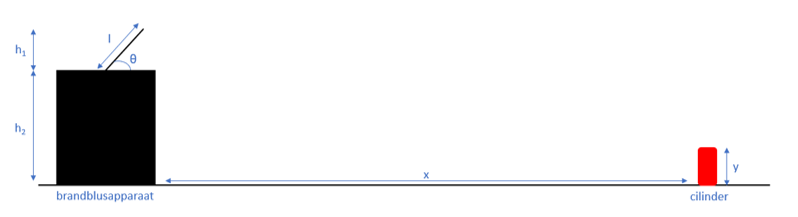
\includegraphics[width = 1 \textwidth]{schematische voorstelling water LATEX}
	\caption{Schematische voorstelling van de opstelling}
	\label{schematische voorstelling}
\end{figure}

\begin{figure} [h!]
	\centering
	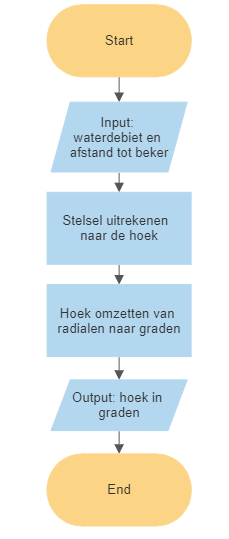
\includegraphics[width = .2 \textwidth]{flowchart_hoekV}
\cprotect\caption{Flowchart van de functie \verb*|hoekV(waterDebiet,afstandBeker)|}
	\label{flowchart_water}
\end{figure}




\subsection{Stoppen met water spuiten}
\subsubsection{Berekening}
Wanneer de hoeveelheid water nodig om een brand te blussen bekend wordt gemaakt en we een foutenmarge uit een handvol experimenten hebben berekend zullen we de hoeveelheid te spuiten water aan onze code kunnen toevoegen. De foutenmarge zal een gemiddelde zijn van water die naast het doelwit terecht komt bij de proeven. \\
Om zo exact mogelijk te weten hoeveel water het apparaat al heeft uitgespoten, maken we gebruik van de waterflowsensor.
%@jesse mss kan je iets schrijven over hoe je berkent hoeveel water er al is gepasseerd met gebruik van de waterflowsensor



\subsubsection{Code}
\begin{figure} [!h]
	\centering                 
	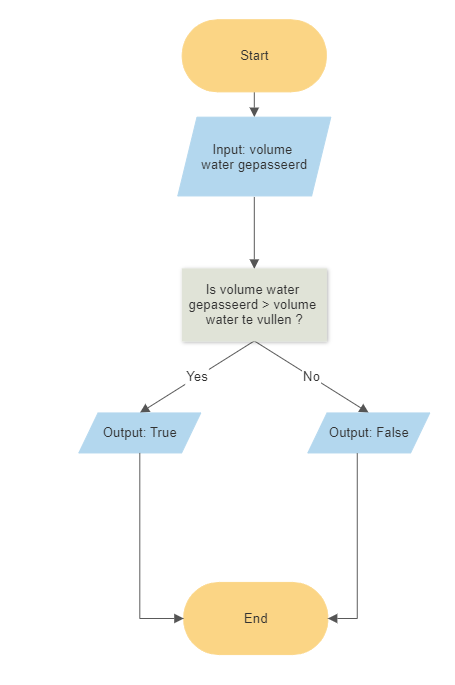
\includegraphics[width = .3 \textwidth]{flowchart_stoppenPompen}
\cprotect\caption{Flowchart van de functie \verb|stoppenPompen()|}
\end{figure}





\subsection{Camera}
\subsubsection{Berekening}
Omdat het gezichtsveld van de camera niet het volledige bestrijkingsgebied omvat (zie figuur \ref{bestrijkingsgebied}), hebben we besloten de camera te laten meedraaien met het draaiende platform en het bestrijkingsgebied van links naar rechts te analyseren. \\

We kunnen de afstand \(d\) van een object tot de camera vinden met de formule \ref{camera}, waarbij \(b_w\) de werkelijke breedte van een object is en \(b_s\) de breedte van het object op het beeld van de camera in \(cm\) (berekend door het aantal pixels in de x-richting te vermenigvuldigen met \(0.02645833333\)). \(f\) is de focal lengte van de camera, dit is eigen aan ieder toestel en werd door ons experimenteel vastgesteld dor dezelfde formule \ref{camera} te gebruiken, maar ze om te vormen naar \(f\) en een object op een gekende afstand te plaatsen en van meerdere waarnemingen het gemiddelde te nemen. 
\begin{equation} \label{camera}
	d = f * \frac{b_w}{b_s}
\end{equation}

Een andere manier om de afstand \(d\) te berekenen is door de hoek te meten tussen de middelste pixel \(p_m\) en buitenste pixel \(p_b\) van het beeld. Dit doen we door de absolute waarde te nemen van het verschil van \(p_m\) en \(p_b\). Deze waarde vermenigvuldigen we met \(gpp\). \(gpp\) staat voor graden per pixel en wordt bekomen door de breedte van het gezichtsveld van de camera (hier 60°) te delen door de breedte van het beeld (640 pixels). De uiteindelijke uitkomst is de hoek \(\alpha\). Om daarmee de afstand te berekenen gebruiken we de formule:
\begin{equation} \label{camera_2}
	d = \frac{b_w}{2} * tan(\alpha)
\end{equation}

\begin{figure} [h!]
	\centering                
	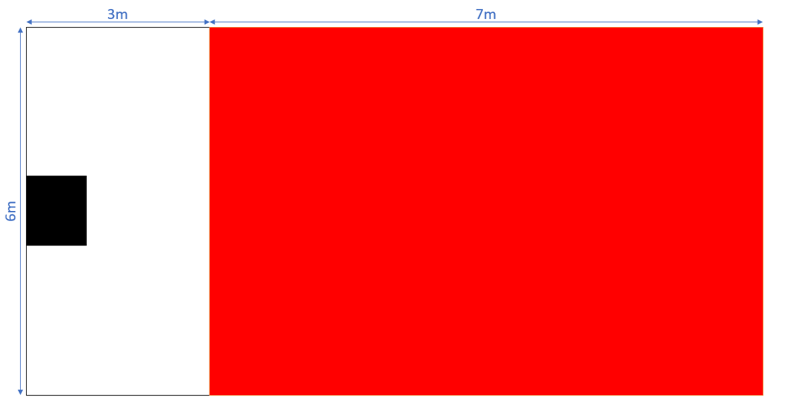
\includegraphics[width = .5 \textwidth]{schematische voorstelling bestrijkingsgebied LATEX}
	\caption{Schematische voorstelling van het bestrijkingsgebied (rood) met het blusapparaat zwart gekleurd}
	\label{bestrijkingsgebied}
\end{figure}

\subsubsection{Code}
In python werd een programma geschreven dat de afstand tot een object kan inschatten aan de hand van camerabeelden. Het kan de beelden vastgelegd door een webcam analyseren dankzij het gebruik van cv2. Daarna zet het het beeld om van BGR (blue-green-red) naar HSV (hue-saturation-value), waardoor we een boven- en onderlimiet kunnen opleggen voor het kleur die we wensen te behouden, hier is dit rood. De output is een zwart beeld waarbij enkel objecten met de gewenste kleur met wit omlijnd zijn.\\
De camera is vastgemaakt op het roterend platform (zie figuur \ref{ontwerp}) waarbij het beeld parallel staat met de arm. We laten dus de camera meedraaien en analyseren zo het volledige bestrijkingsgebied van links naar rechts. Wanneer een object wordt opgemerkt en de hoek waaronder het object zich bevind tussen twee bepaalde waarden ligt (nu nog -1° en 1°), dit wil zeggen dat het in het midden van het beeld staat, wordt de afstand \(d\) tot het object berekend. Dit gebeurt op 2 manieren: 
\begin{itemize}
	\item We maken gebruik van formule \ref{camera}
	\item We maken gebruik van formule \ref{camera_2}
\end{itemize}
We benutten beide methoden en nemen het gemiddelde van de twee uitkomsten voor \(d\) en verkrijgen op die manier de meest accurate waarde voor \(d\).


\begin{figure} [!h]
	\centering
	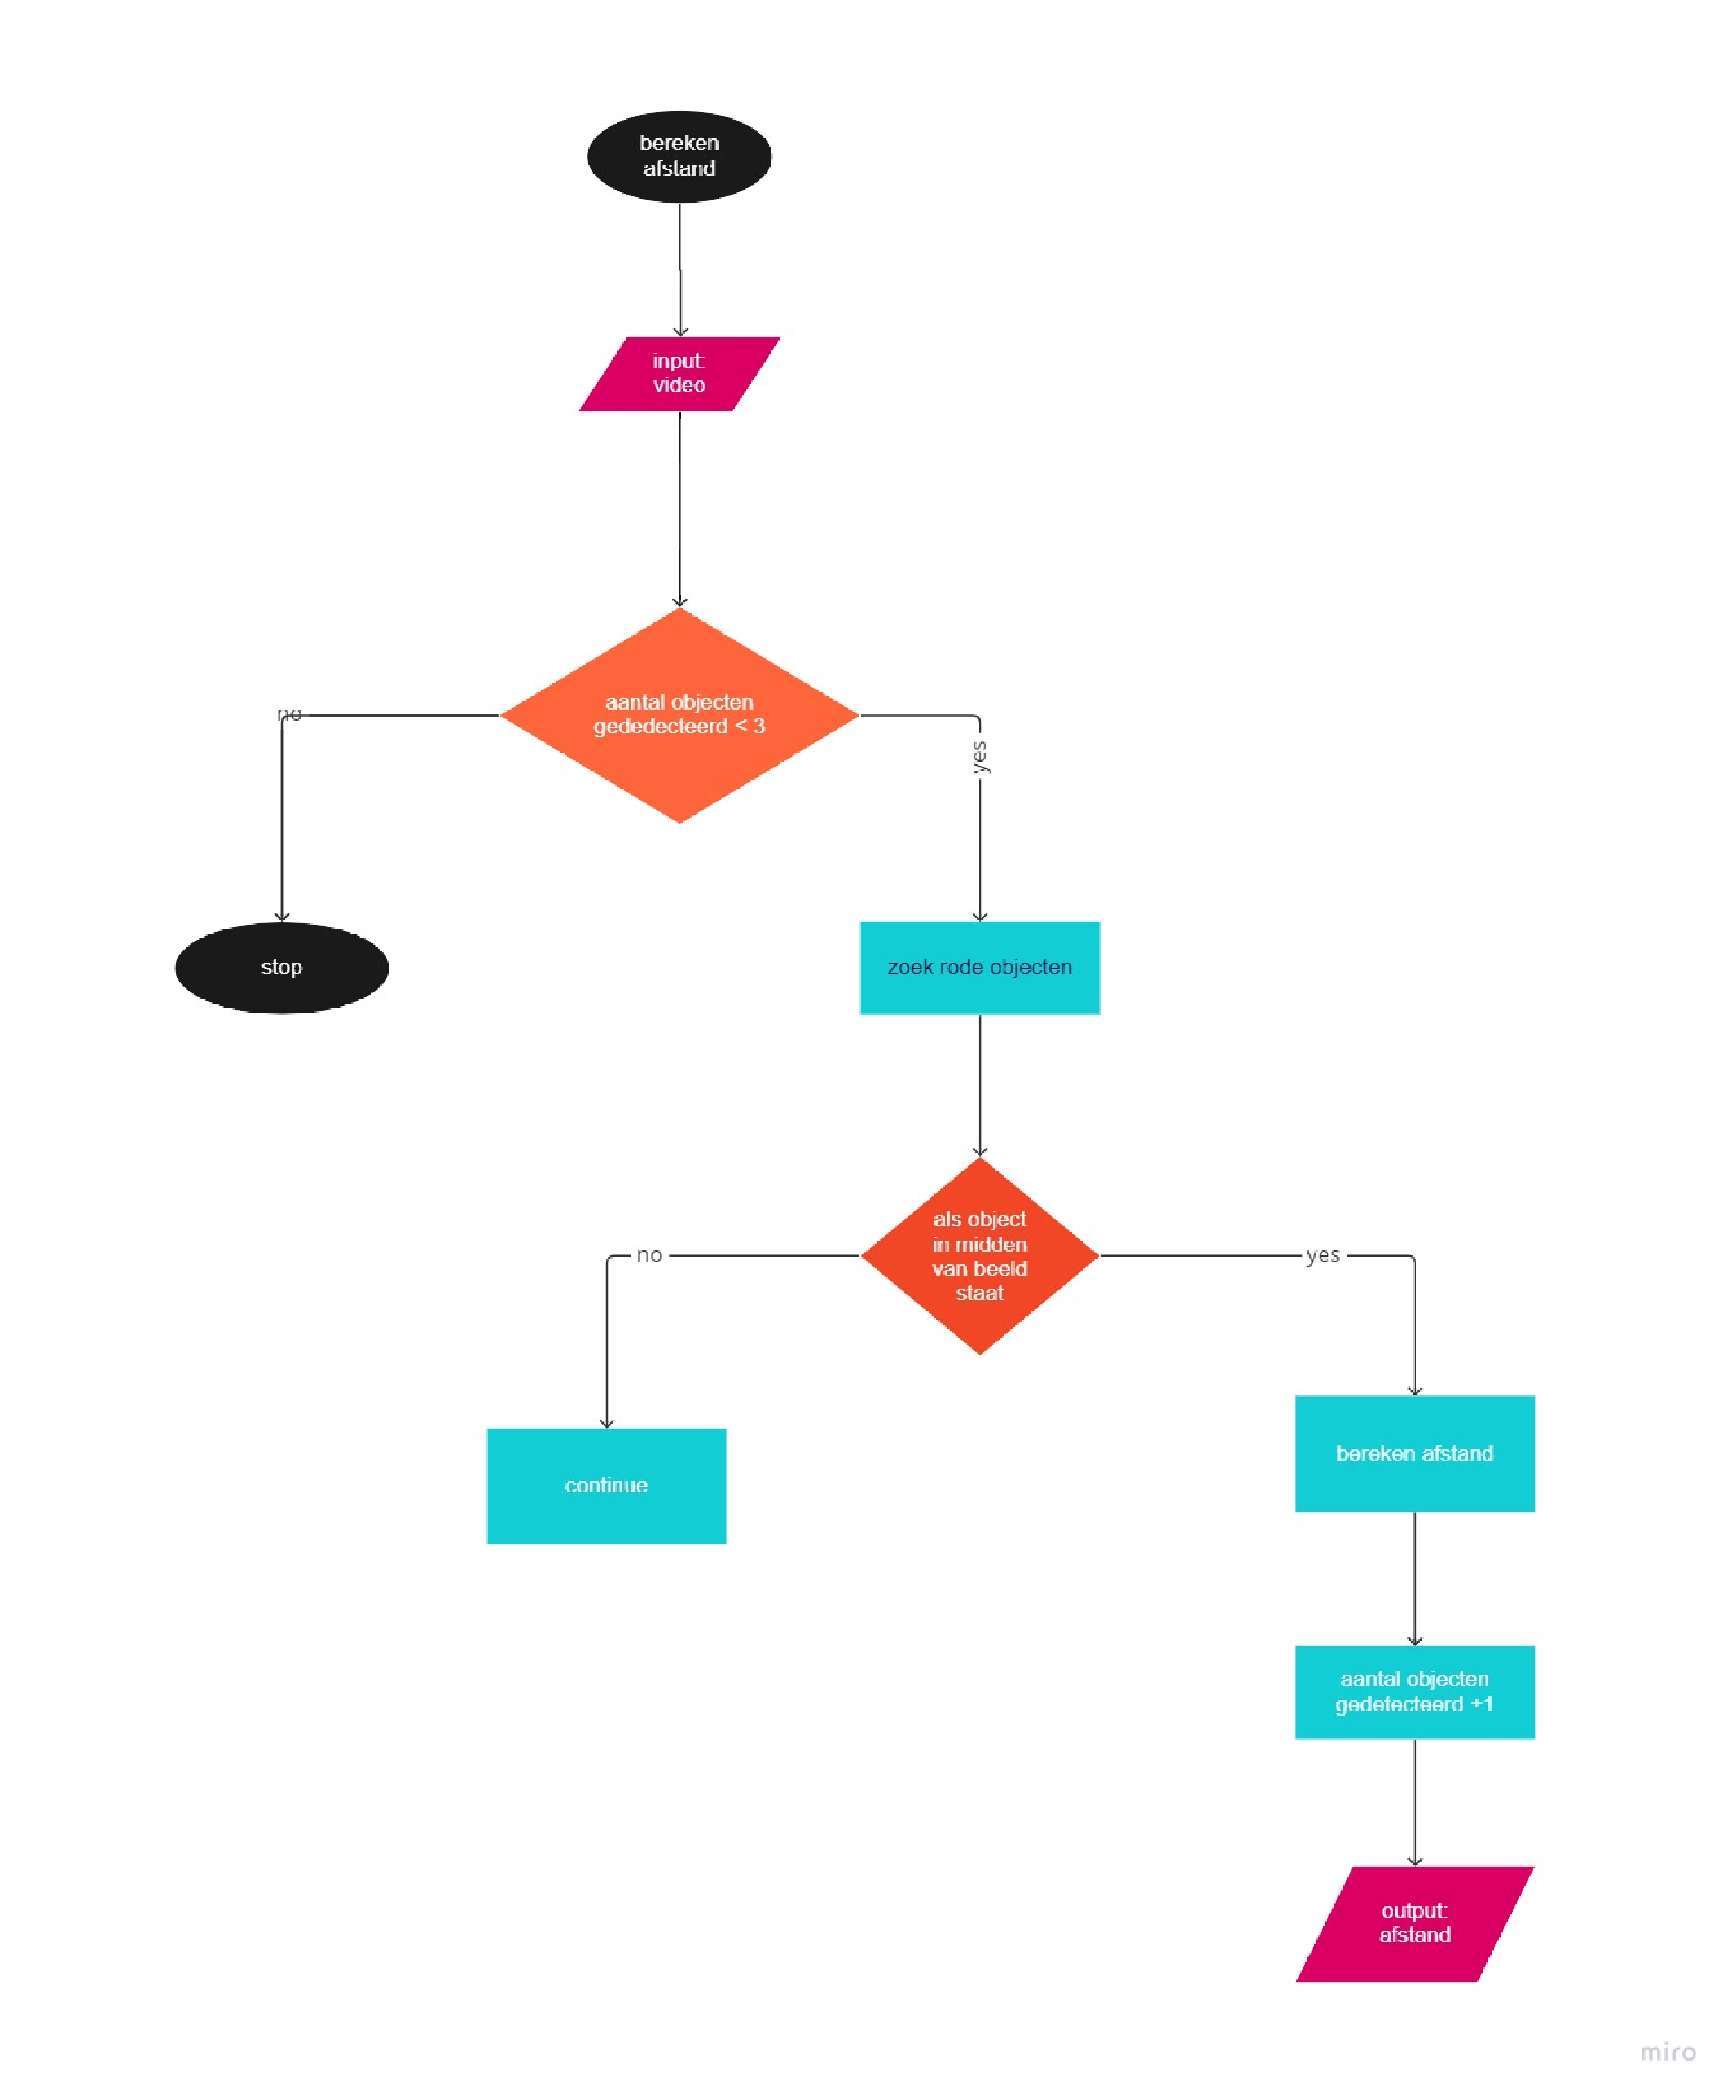
\includegraphics[width = 0.8 \textwidth]{flowchart afstand berekenen.pdf}
\cprotect\caption{Flowchart van de functie \verb*|berekenen_afstand()|}
\end{figure}
 
%\subsection{Lengte van de arm}
%\subsubsection{Berekening}
%@jesse mss kan je je berekeningen over de beste lengte van de arm toevoegen?


\section{Planning}
Op de pagina hieronder is onze taakstructuur te vinden. De eerste taak, het verkennen van de opdracht, is al voltooid. Ons CAD model is bijna af en we zijn al begonnen met het coderen van de microcontroller en PC alsook met de bouw van het geraamte van ons apparaat. We hopen met een prototype klaar te zijn tegen 28 april 2023, zodat we daarna kunnen beginnen met testen en nodige aanpassingen kunnen maken.
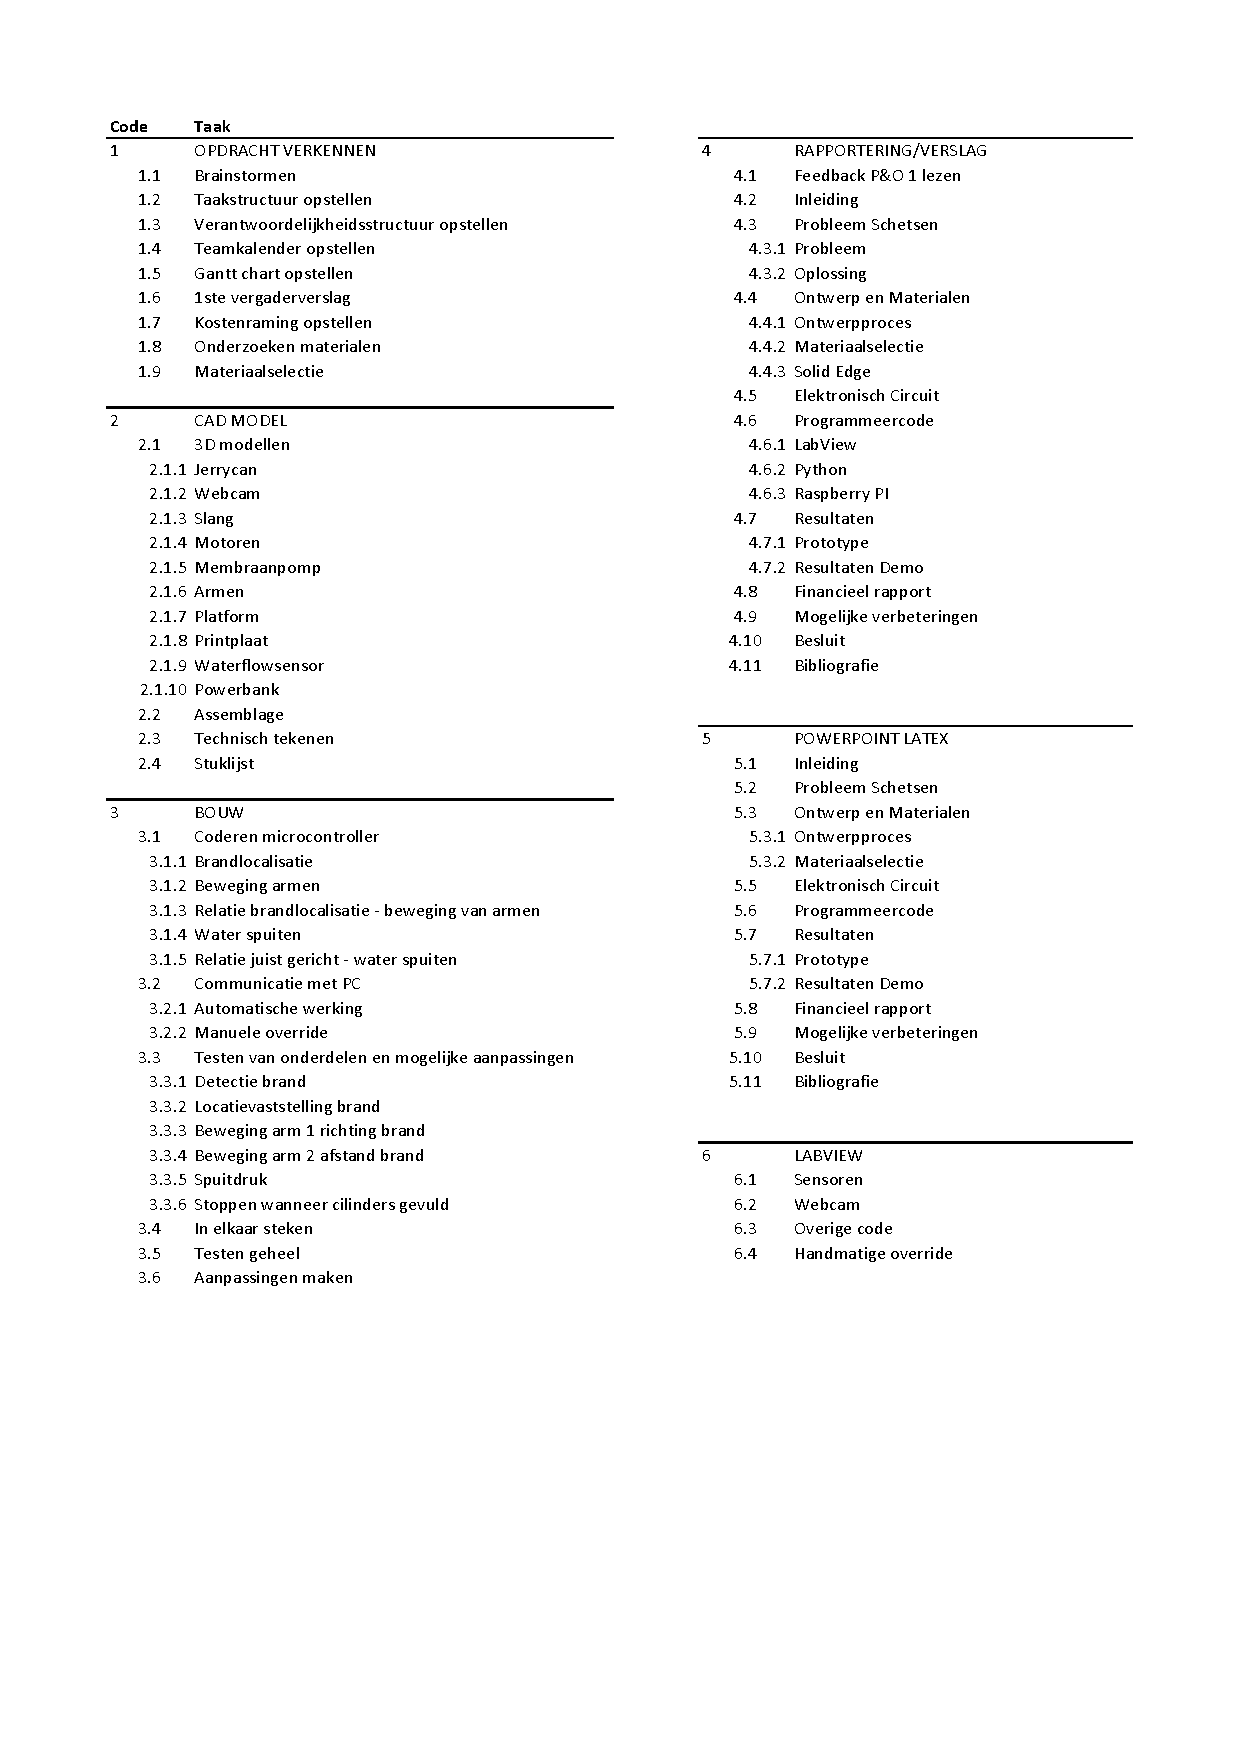
\includepdf{taakstructuur_LATEX_2.pdf}


\end{document}
